%-------------------------------------------------
% FileName: chapt-4.tex
% Author: MrLQQ
% Date: 2021-10-7
% Description: 第4章
% Others: 
% History: origin
%------------------------------------------------- 


% 断页
% \clearpage
\chapter{总体设计}

\section{系统总体设计}
描述根据系统的需求分析,确定系统的功能模块构成。

\section{功能模块设计}
说明各个功能模块的数据结构和实现算法。


C源代码
\begin{clan}
    #include <stdio.h>  
    int main()                  //main 入口函数  
    {  
        printf("Hello,World!"); //printf 函数打印  
        return 1;               //函数返回值  
    }   
\end{clan}


matlab源代码
    \begin{matlab}
    function F=random()
    a=[1 2];
    Prob=[0.99 0.01];
    F=randsrc(1,1,[a;Prob]);

    areas=[]
    for i=1:100
    x=unifrnd(0,10,[1,100]);
    y=unifrnd(0,10,[1,100]);
    frequency=sum(x<=1)+sum(y<=1);
    area=100*frequency/100;
    areas=[areas,area];
    end
\end{matlab}


python源代码
\begin{python}
    from multiprocessing import Pool
    import os, time, random

    def long_time_task(name):
        print('Run task %s (%s)...' % (name, os.getpid()))
        start = time.time()
        time.sleep(random.random() * 3)
        end = time.time()
        print('Task %s runs %0.2f seconds.' % (name, (end - start)))

    if __name__=='__main__':
        print('Parent process %s.' % os.getpid())
        p = Pool(4)
        for i in range(5):
        p.apply_async(long_time_task, args=(i,))
        print('Waiting for all subprocesses done...')
        p.close()
        p.join()
        print('All subprocesses done.')
\end{python}




C++源代码
\begin{cpp}
    #include <iostream>               //std::cout 要用到的头文件  
    #include <stdio.h>                //标准输入输出头文件  

    int main()  
    {  
        printf("Hello,World!--Way 1\n");    //printf 语句打印  
        puts("Hello,World!--Way 2");        //puts 语句  
        puts("Hello," " " "World!--Way 3"); //字符串拼接  
        std::cout << "Hello,World!--Way 4" << std::endl; //C++ 教科书上写法  
        return 1;                                        //作为注释  
    }  
\end{cpp}




Csharp源代码
\begin{clan}
    //FileName: HelloWorld.cs  
    using System;  
    class TestApp  
    {  
        public static void Main()  
        {  
            Console.WriteLine("Hello,World!");  
            Console.ReadKey();  
        }  
    }   
\end{clan}

java源代码
\begin{java}
    #FileName: HelloWorld.java 
    #如果有 public 类的话,类名必须和文件同名,注意大小写   
    public class HelloWorld   
    {  
        #Java 入口程序,程序从此入口  
        public static void main(String[] args)  
        {  
            #向控制台打印一条语句  
            System.out.println("Hello,World!");  
        }  
    }  
\end{java}


js源代码
\begin{javascript}
    var sys = require("sys");    #导入需要的 sys 模块  
    sys.puts("Hello,World!");    #调用里面的 puts 函数来打印字符串  
\end{javascript}

php源代码
\begin{php} 
    <?php  
        echo "Hello,World!";            //打印语句  
        echo "The first php program!";  //打印语句  
        echo phpinfo();                 //phpinfo()系统函数,输出环境信息  
    ?>    
\end{php}


go源代码
\begin{gogo}

    //filename: hello.go
    package main 
    import (
        "fmt"
        "os"
    )
    func main(){ //这个 { 不能另起一行
        fmt.Println("hello world!")
    }
\end{gogo}

html源代码
\begin{html}
    <!DOCTYPE html>  
    <html>  
        <body>  
            <h1>This is the first program!</h1>  
            <p>Hello,World!</p>  
        </body>  
    </html>
\end{html}

xml源代码 
\begin{xml}
    <?xml version="1.0"?>
    <class name="Student" table="student">
        <id name="id" column="id" ></id>
        <property name="name" column="name" ></property>
        <property name="age" column="age" ></property>
    </class> 
\end{xml}

sql源代码 
\begin{sql}
    SQL> CREATE TABLE MESSAGE (TEXT CHAR(15));            #创建表  
    INSERT INTO MESSAGE (TEXT) VALUES ('Hello, world!');  #插入表  
    SELECT TEXT FROM MESSAGE;                             #查询表  
    DROP TABLE MESSAGE;                                   #删除表               
    Table created.   
\end{sql}

tex源代码 
\begin{tex}
    \begin{figure}[H]
        % 居中
        \centering 
        % width=.5\textwidth 文档宽度的0.5
        % fig1图片放在img目录下,在此处引用无需img/前缀和图片格式后缀(png, jpg等)
        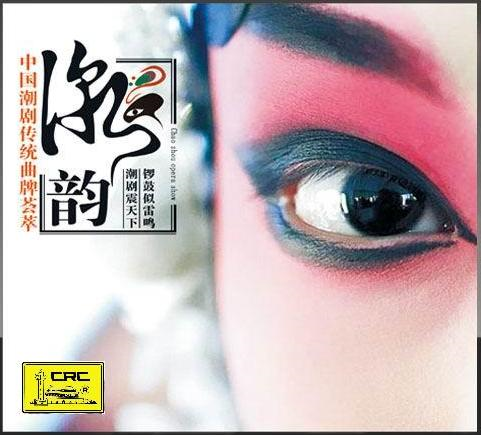
\includegraphics[width=.5\textwidth]{fig1} 
        % label紧接caption之后,用于引用
        \caption{这是一个图}
        \label{fig:single}
    \end{figure}
\end{tex}